\section{Algoritmo Progettato}
In questa sezione saranno illustrati sequenzialmente i passi effettuati dal software. I passi sono  seguenti:
\begin{itemize}[noitemsep]
    \item Caricamento dataset
    \item Caricamento lista RFD
    \item Ordinamento delle RFD
    \item Query Estesa
    \item Query Rilassata
\end{itemize}
\begin{figure}[H]
\centering
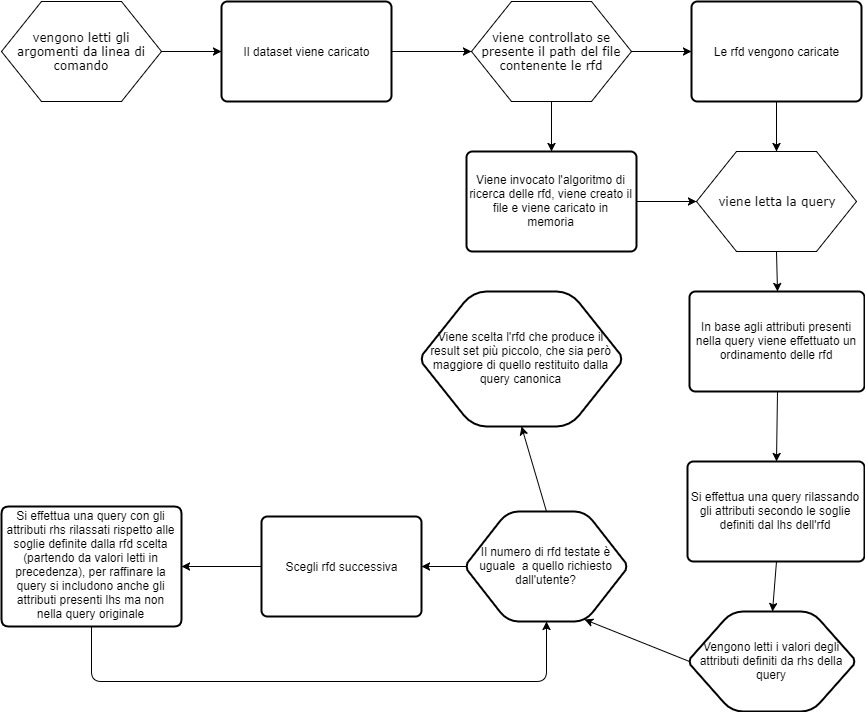
\includegraphics[width=\textwidth,height=\textheight,keepaspectratio]{images/Flowchart.jpg}
\caption{Flowchart}\label{fig:4}
\end{figure}
\paragraph{Caricamento Dataset}
Il primo passo da effettuare è quello di caricare il DataSet in formato csv. Il separatore che di norma può essere costituito da un carattere a scelta è stato impostato come carattere ";".\\ Il DataSet può contenere vari tipi di dati: float, int, stringhe e date.
La struttura dati utilizzata per contenere i dati è quella del pandas.Dataframe , contenuta nel package Pandas\footnote{Pandas è una libreria software scritta per il linguaggio di programmazione Python .È adibita alla manipolazione e l'analisi dei dati. In particolare, offre strutture e operazioni di dati per la manipolazione di tabelle numeriche e di serie temporali. }. \\Il Dataframe di Pandas è una struttura dati tabulare bidimensionale variabile in formato e con assi etichettati (righe e colonne). Le operazioni vengono effettuate sulle righe e sulle colonne. 
\paragraph{Carimento lista RFD}
Il secondo passo consiste nel caricare la lista di RFD. L'utente può passare il path del file contenente le RFD, altrimenti viene invocato un algoritmo di ricerca di RFD sul DataSet indicato.
Nel caso in cui venga passato il path, il formato del file deve essere di tipo csv, con carattere di separazione uguale a ";"\footnote{In realtà è stato implementato un sistema capace di riconoscere ed utilizzare un qualsiasi carattere di separazione}.
Dato che ogni RFD può avere un attributo diverso come parte RHS , si è scelto di utilizzare una particolare notazione:
\begin{table}[H]
    \centering
    \begin{tabular}{l l l l l }
     RHS & $attr_1$ & $attr_2$ & $attr_{\ldots}$ & $attr_n$ \\
    $attr_{k}$ & $s_{12}$ & $s_{13}$ & $s_{\ldots}$ & $s_1n$  \\
    $attr_{j}$ & $s_{22}$ & $s_{23}$  & $s_{\ldots}$ & $s_{2n}$\\
    $attr_{p}$ & $s_{\ldots1}$ & $s_{\ldots3}$  & $s_{\ldots}$ & $attr_{r}$\\
    $s_{m1}$ & $s_{m2}$ & $s_{m3}$ & $s_{\ldots}$ & $s_{mn}$\\
    \end{tabular}
    \caption{Pandas Dataframe contenente le soglie delle RFD}
    \label{tab:RFD_notation}
\end{table}

La prima colonna del Dataframe contiene non una soglia bensì il nome dell'attributo che funge da RHS in quella RFD.
\\
Se l'utente non fornisce il path del file, o se il file non viene trovato, il software richiama l'algoritmo di ricerca delle RFD. Il path del Dataset viene passato all'algoritmo di RFDD\footnote{Relaxed Functional Dependencies Discovery} , dopo aver elaborato restituisce una Dataframe contenente le RFD, le quali vengono salvate su file e successivamente caricate in memoria.
\paragraph{Ordinamento delle RFD}
Una volta caricata la lista di query è necessario effettuare una pulizia sui dati.
Vengono eliminate le RFD che possiedono valore "NaN" su attributi che sono presenti nella query, dopodiché vengono eliminate le RFD dove nel lato RHS è presente un attributo della query \footnote{Utilizzare una RFD di questo tipo significherebbe utilizzare una dipendenza funzionale rilassata banale, la quale non porta alcuna informazione aggiuntiva}
\begin{table}[H]
    \centering
    \begin{tabular}{l l l l l }
     RHS & $attr_1$ & $attr_2$ & $attr_{\ldots}$ & $attr_n$ \\
    $attr_{k}$ & $s_{12}$ & $s_{13}$ & $s_{\ldots}$ & $s_1n$  \\
    $attr_{j}$ & $s_{22}$ & $s_{23}$  & $s_{\ldots}$ & $s_{2n}$\\
    $attr_{p}$ & $s_{\ldots1}$ & $s_{\ldots3}$  & $s_{\ldots}$ & $attr_{r}$\\
    $s_{m1}$ & $s_{m2}$ & $s_{m3}$ & $s_{\ldots}$ & $s_{mn}$\\
    \end{tabular}
    \caption{Pandas Dataframe contenente le soglie delle RFD}
    \label{tab:RFD_notation}
\end{table}
Dopo aver effettuato questa pulizia le RFD vengono ordinate. 
\newline
C'è stata molta indecisione riguardo l'implementazione dell'ordinamento, in quanto non è stata trovata una dimostrazione formale che ci indicasse quale metodo fosse il più efficace.
L'obiettivo è stato quello di trovare un algoritmo che ordinasse le RFD dando precedenza a quelle che producono Result Set non troppo ampi.
\\
Dopo vari test abbiamo pervenuto che il metodo più efficacie fosse quello di ordinare le RFDs prima in ordine decrescente rispetto al numero di attributi con valore "NaN" e poi in ordine crescente di soglia rispetto agli attributi presenti nella query. 
L'ordinare secondo soglie più piccole indica che quelle RFD agiscono su range ridotti, indicativamente ciò significa che rispetto ad un range più ampio un range di dimensioni ridotte include meno dati .In realtà può capitare che in un range di un DataSet vi sia una forte aggregazione di dati , superiore a tutti gli altri dati presenti nel Dataset. Ad esempio preso un Dataset che possiede un attributo altezza possiamo avere i seguenti valori
\begin{table}[H]
    \centering
    \begin{tabular}{l }
    altezza \\
    170 \\
    171 \\
    172 \\
    171 \\
    169 \\
    170 \\
    173 \\
    170 \\
    169 \\
    158 \\
    165 \\
    152 \\
    \end{tabular}
    \caption{Esempio di valori su attributo altezza}
    \label{tab:height_list}
\end{table}
In questo caso se abbiamo due range $[169,172]$ e $[140,165]$, l'intuizione ci dice che il primo range essendo il più piccolo dovrebbe includere meno dati, invece guardando dalla lista si può notare che il primo range contiene 8 valori ed il secondo solo 3.
Ciò capita abbastanza raramente , infatti nei test effettuati questo principio di ordinamento ha restituito quasi sempre i risultati migliori.
Per aumentare l'efficacia dell'ordinamento abbiamo ritenuto necessario dare precedenza alle RFD che nel lato LHS possiedono un numero di attributi il più simile possibile agli attributi presenti nella query.
Nella tabella sottostante viene mostrata parte di una lista di RFD ordinata \footnote{L'ordinamento è stato effettuato in base ad una query eseguita dall'utente, in questo caso la query è SELECT * FROM dataset{\_}string WHERE height=169}:
\begin{table}[H]
    \centering
    \begin{tabular}{l l l l l l l l}
        & RHS & age & height & shoe{\_}size & weight \\
        \hline
    0 & shoe{\_}size & NaN & 0.0 & 1.0 & NaN \\
    1 & weight & NaN & 0.0 & 0.0 & 1.0 \\
    2 & shoe{\_}size & 3.0 & 0.0 & 0.0 & NaN \\
    3 & weight & 6.0 & 1.0 & NaN & 4.0 \\
    4 & weight & NaN & 1.0 & 1.0 & NaN \\
    5 & shoe{\_}size & 6.0 & 1.0 & 1.0 & NaN \\
    6 & shoe{\_}size & NaN & 1.0 & 1.0 & 4.0 \\
    7 & shoe{\_}size & NaN & 1.0 & 0.0 & 2.0 \\
    8 & age & 6.0 & 1.0 & 0.0 & NaN \\
    9 & age & 5.0 & 1.0 & 1.0 & NaN \\
    \ldots & \ldots & \ldots & \ldots & \ldots & \ldots \\
    \end{tabular}
    \caption{Parte di una lista di RFD ordinata}
    \label{tab:ord_rdf}
\end{table}

\paragraph{Query Estesa}
D'ora in poi tutta la procedura descritta da qui in avanti verrà iterata per un numero di RFD pari ad un valore definito dall'utente. \footnote{In caso in cui l'utente lasci il campo vuoto, l'iterazione viene effettuata per ogni RFD presente nella lista}
Viene selezionata la i-esima RFD con $i\in[1,n]$. 
Si vanno a considerare gli attributi della RFD che siano presenti nella query\footnote{In questo momento si considerano solo gli attributi in LHS}, si prendono le soglie e si effettua una nuova una query estesa $Q_2$
Ad esempio supponendo che la query iniziale sia: \\~\\ \centerline{SELECT * FROM dataset{\_}string WHERE height=169} \\~\\ e che la RFD selezionata sia: \\~\\ \centerline{$(height \leq 0.0)  \rightarrow(shoe_size \leq 0.0)$} \\~\\
Viene effettuato un controllo sul tipo di valori degli attributi della query,
si vanno a identificare tipi string, int e float, questa identificazione serve a specificare quale funzione di distanza bisogna applicare durante l'estensione della query.
Dato che $height$ è un attributo di tipo numerico, si vanno a prendere tutti i valori che differiscono di 0 dal valore iniziale inserito dall'utente. In questo caso la query estesa $Q_2$ resta uguale a $Q_1$: \\~\\ 
\centerline{SELECT * FROM dataset{\_}string WHERE height =169} \\~\\
Effettuando una nuova interrogazione con la query $Q_2$ otteniamo un Result Set che sarà di sicuro $\geq$ del Result Set restituito dall query iniziale.
In questo caso entrambe le query restituiscono questo risultato: \newline 
\begin{table}[H]
    \centering
    \begin{tabular}{l l l l l l l l}
    n.row   & height & weight & shoe{\_}size & age \\
    \hline
    5 & 169 & 73 & 38 & 49 \\
    \end{tabular}
    \caption{Result Set restituito sia dalla query $Q_1$ e sia dalla query $Q_2$ }
    \label{tab:sta_ext_result_set}
\end{table}
\paragraph{Query Rilassata}
In questa procedura viene effettuato il vero e proprio rilassamento, scambiando gli attributi della query con attributi definiti dalla parte RHS della RFD selezionata (vedi Appendice [perfezionamento con lhs]).
Inizialmente si effettua una raccolta dei valori nel dataset, si selezionano solo gli attributi che sono presenti in RHS. Viene mantenuta una struttura dati\footnote{In questo momento lo definiamo come un set} per ogni tupla restituita dal dataset (vedi Appendice [perfezionamento combinazioni]). 
Per ogni Set vengono rilassati i valori in base alle soglie contenute nella RFD, il risultato sarà una serie di SET che contengono dei range più ampi.
È quindi possibile effettuare $k$ query rilassate, ottenendo vari Result Set. La loro unione andrà a costituire il Result Set finale che sarà restituito in output.
Riprendendo l'esempio riportato nel paragrafo precedente, vengono raccolti i dati sui valori presenti in RHS, in questo caso vi è solo l'attributo shoe{\_}sie \footnote{In realtà in RHS vi è sempre un unico attributo, la query viene rilassata con più attributi in quanto si esegue un perfezionamento vedi  Appendice [perfezionamento combinazioni]} che viene rilassato di una soglia pari a 0. Dato che la query estesa $Q_2$ ha restituito una sola tupla, verrà rilassato un unico valore. La query rilassata $Q_3$  è : \newline 
\centerline{SELECT * FROM dataset{\_}string WHERE shoe{\_}size=38}
\newline
Per la proprietà delle RFD (vedi Appendice Proprietà RFD) il Result Set restituito sarà $\geq$ del Result Set restituito dalla query estesa $Q_2$.

In questo caso il Result Set è uguale a :
\begin{table}[H]
    \centering
    \begin{tabular}{l l l l l l l l}
    n.row  & height & weight & shoe{\_}size & age \\
    \hline
    0  & 175 & 75 & 39 & 41 \\
    1  & 169 & 73 & 38 & 49 \\
    2  & 170 & 65 & 39 & 30 \\
    \end{tabular}
    \caption{Result Set restituito sia dalla query $Q_3$ }
    \label{tab:relax_result_set}
\end{table}

Dato che questa procedura viene effettuata per un numero N di RFD, viene effettuato un confronto in modo tale da restituire il Result Set che che sia il meno ampio possibile \footnote{Vengono scartati i Result Set che hanno cardinalità uguale ad Result restituito dalla query iniziale}.


